%\newpage
\section{Conclusions}

Several possible variants of SOA implementation were covered in this work.
Some of them are mature and standardized tools which are used in many production
systems nowadays.
Another ones are lightweight and beautiful alternatives to the first group. They
can be  used even in the small microcontroller devices. 
Their specifications does not tie a programmer to work with a limited specific
set of technologies. 
Some of covered tools can be used in any environment and support all creativity
of the developers. 
JSON and XML, the ideas of RPC, they all can be used in many various ways.

Author was trying to analyse all of them in his research.
This work chosen some comparison of SOA implementations and related technologies
is the context of the embedded systems.
Some technologies were chosen for the trial.
The choice of the technologies  does not mean that they are the best and the
only suitable solution for the application described here.
Author's  aim was to show that it is possible to create the systems of small
devices using lightweight protocols and data structures.

Some specific application field was chosen as an example in this work.
Lets watch how it was realized and overview the results.

\subsection{Results}

There was a defined goal of this work: make a research of available
machine-to-machine communication techniques and deliver a functional system
prototype to fulfill some business needs.

Author has a freedom of choosing any suitable technology and was limited only
with the available hardware platform. 
This work can be characterize as a research activity of detecting possible
facilities, not than an implementation of specific task of interconnecting
a mobile phone and the coffee machine.
There should be a goal to reach, some problem which needs a solution in order to
start watching around. 
I have defined this abstract task and decided to make a
case study about it.

One of multiple ways how to design a client-server system is the
SOA. Services are self-describing and open components, which use standard
communication schemes. 
Author of this work was inspired by this approach and have created a SOA
based system.


This paper contains a research of different technologies that help to implement
services on the devices.
It is unable to find and analyse all possible solutions. The most popular and
open approaches were analysed instead. 
Author has chosen a concept of remote procedure calls and found a simple
and lightweight solution of JSON-RPC. 

I had no experience of programming microcontrollers before. The company, where i
was doing my university internship, provided me one specific microcontroller
family and my task was to learn how it can be applied. To find out the
hardware possibilities you need to study the  architecture of a specific
devices.
This work became for me not only a research project, but  a complete
microcontroller practical course.
I have learned how to use different development tools and STM32F1 and other ARM
Cortex-M3 microcontroller hardware platform features, exercised low level C
programming and even soldered wires on development boards to repair boundary
scan debugger.
This was done only by myself with the help of internet resources
and other information sources.
This was the largest laboratory work i have ever experienced.

A small remote service was finally implemented on a STM32F103ZE microcontroller. 
This server is able to response for remote client requests and provide some
useful services.
This device is a proxy bridge between client application and coffee machine
hardware.
Only a few set of functions were implemented, but this functionality reflects all
the architecture features.
It is able to determine the structure of this system by tracing how a
single RPC request is transferred between different system modules..

This solution uses embedded realtime operating system FreeRTOS, so i was
involved in a development of a parallel and multitasking system. 
Server program consists of parallel tasks, which are communicating to each other
and process incoming requests. Internals are implemented as chain of
processing units, which pass work to each other.

The client side of application is designed as a Java library that can be used
in any kind of client application. It provides remote device methods and handles
all communication between the client code and embedded service server.

This library  is used inside the Android demo application, that is executed on
the mobile phone or tablet.
The Android program was designed to be an example application case. 
This provides some controls over the remote coffee machine. 


The goal of this work was achieved.
This was a research of a big bunch of technologies: embedded hardware related
highly constrained and optimized software was studied together with  modern
internet technologies that connect billions different machines.

Lots of new things and interesting computer science approaches were found during 
accomplishing the tasks and information mining.
Obtained experience and knowledge would help me to
deliver more quality products in future and not to make those mistakes that
every young computer system engineer does.

\subsection{Future work}
This small implementation of client-server application connects together only
two devices. 
This does not define any additional methods how to find
devices in a network and connect other devices.
This is only an abstract service architecture that was designed to be universal.

There is no security, addressing, discovery and quality of service. 
It requires some reliable transport protocol stack that covers data transferring
from physical communication layer up to application layer.

In order to become a real world product and be integrated to other systems 
there should be dedicated connectivity requirements.
Devices should be connected in some standard way. 

Most of reviewed information sources covered the development of embedded services in
context of internet and TCP/IP networks.

I see the next development cycle of this architecture to be the integration to
the Internet of Things.
Many research groups are working on developing distributed communication for
small embedded devices and wireless sensor networks on the Internet. 
Their work papers include keywords like 6LoWPAN, IEEE 802.15.4, IPv6, RPL,  UDP, COAP, RESTful embedded services.

\autoref{fig:future_technologies} shows how this technologies could be applied.

\begin{figure}[H]
        \centering		  
		  \begin{tabular}{c}
			\subfloat[Optimized IP protocols]{
				\label{fig:optimized_ip_stack}
				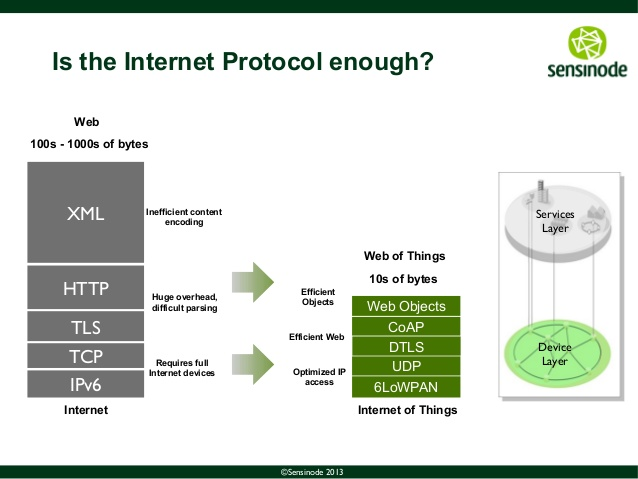
\includegraphics[width=0.5\textwidth]{../images/optimized_ip.jpg}
			} \\
			\subfloat[RESTful Web things Things architecture]{
				\label{fig:restful_wot}
				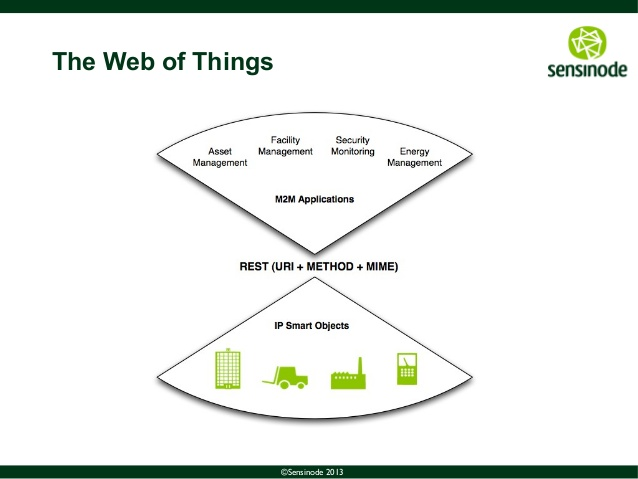
\includegraphics[width=0.5\textwidth]{../images/restful_WoT.jpg}
			} \\
			\subfloat[RESTful temperature sensor usage example]{
				\label{fig:restful_sensor}
				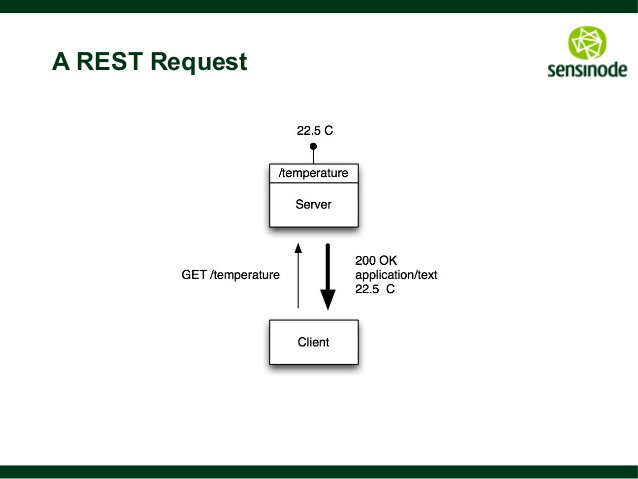
\includegraphics[width=0.5\textwidth]{../images/restful_temperature_sensor.jpg}
			} 
		  \end{tabular}        
        \caption{Optimized internet technologies for networked embedded systems~\cite{iot_standards,CoAP_Tutorial}}
        \label{fig:future_technologies}
\end{figure}


During this research i have found a project named Contiki.
Contiki is an open source operating system for networked, memory-constrained systems with a particular focus on low-power wireless Internet of Things devices.
Examples of where Contiki is used include street lighting systems, sound monitoring for smart cities, radiation monitoring systems, and alarm systems.\footnote{\url{http://www.contiki-os.org/}}

This project supports  very resource efficient  full IP networking\footnote{ uIP TCP/IP Stack from Adam Dunkels. See ~\cite{Dunkels07programmingmemory-constrained} } and is optimized for tiny systems, having only a few kilobytes of memory available. 
This is a good candidate to be the main technology of this kind of system we have been developed here.

Our design could be rewritten for the Contiki OS and we could migrate to the hardware used in wireless sensor networks.
This could be a very tiny chip with some wireless interface onboard.
It is able to build very low-power and low-cost embedded web service  using this technology stack.

This kind of work requires another exhaustive research and laboratory experiments.
This field is the topic of interest of many scientists and companies, who produce networked embedded solutions.
It is quite popular nowadays and there are many use cases and benefits using distributed embedded network computing.

More and more devices gets connected to the internet. 
This technologies could help to improve the quality of our lives by
introducing a network of low-cost and low-power sensors and actuators. 


